% Launchkey 49 MK3 overlays: label strips to print at actual size, cut out and
% lay on the panel next to the controls. Page 1 freak, page 2 grains, page 3 groove,
% page 4 soliton, page 5 aeolian, page 6 raw.
% Build: make overlays.  Labels come from lib/launchkey_ctl.h (freak),
% lib/grains_ctl.h (grains), lib/groove_ctl.h (groove), lib/soliton_ctl.h
% (soliton), lib/aeolian_ctl.h (aeolian) and lib/raw_ctl.h (raw), as on the cheat sheets.
%
% Spacing: the centre-to-centre distances below are NOT measured (Novation
% publishes no panel drawing). Each strip is divided into one cell per
% control by dashed lines: if the strip does not line up, cut along them and
% place each cell on its own, or measure and change these three lengths.
\newcommand{\kp}{22}   % knob 1 -> knob 2, mm (estimate)
\newcommand{\pp}{22}   % pad column -> next pad column, mm (estimate)
\newcommand{\fp}{22}   % fader -> next fader (and fader button), mm (estimate)

\documentclass{article}
\usepackage[a4paper,landscape,margin=0mm]{geometry}
\usepackage[T1]{fontenc}
\usepackage[default]{sourcesanspro}
\usepackage{amssymb}
\usepackage{tikz}
\pagestyle{empty}
\setlength{\parindent}{0pt}

\definecolor{ink}{RGB}{30,30,30}
\definecolor{grc}{RGB}{0,130,120}      % GRAIN page
\definecolor{fxc}{RGB}{30,90,170}      % FX page
\definecolor{ampc}{RGB}{67,160,71}     % amp envelope
\definecolor{modc}{RGB}{230,140,20}    % mod envelope
\definecolor{lfoc}{RGB}{150,60,170}    % LFO
\definecolor{fltc}{RGB}{215,60,50}     % filter
\definecolor{freec}{RGB}{160,160,160}  % unassigned
\definecolor{engc}{RGB}{190,40,110}    % soliton engine parameters

\tikzset{
  cut/.style={draw=black, line width=0.35pt},             % cut here
  sep/.style={draw=black!45, line width=0.3pt, dash pattern=on 1.2mm off 0.8mm},  % cut apart if needed
  lab/.style={font=\fontsize{6.6}{7.4}\selectfont\bfseries, text=ink, align=center, inner sep=0pt},
  note/.style={font=\fontsize{6.4}{7.6}\selectfont, text=black!60, anchor=north west, align=left, inner sep=0pt},
}
\newcommand{\sm}[1]{{\fontsize{5.2}{6}\selectfont\mdseries #1}}
\newcommand{\FX}[1]{\textcolor{fxc}{#1}}
\newcommand{\GR}[1]{\textcolor{grc}{#1}}

% \strip{x}{y}{cells}{pitch}{height}{label list}{caption}: a row of cells of
% width pitch, one per control, left to right. Solid outline, dashed
% separators. The caption sits above the strip, outside the cut.
\newcommand{\strip}[7]{%
  \foreach \t [count=\i from 0] in {#6} {
    \node[lab, text width=\dimexpr #4mm-1.2mm\relax] at ({#1+(\i+0.5)*#4}, {#2+#5/2}) {\t};
    \ifnum\i>0 \draw[sep] ({#1+\i*#4}, #2) -- ++(0, #5); \fi
  }
  \draw[cut] (#1, #2) rectangle ++({#3*#4}, #5);
  \node[note, anchor=south west] at (#1, {#2+#5+0.8}) {#7};}
% \tag{x}{y}{label}: one small label for a single button.
\newcommand{\tag}[3]{%
  \draw[cut] (#1, #2) rectangle ++(17, 7.5);
  \node[lab, text width=16mm] at ({#1+8.5}, {#2+3.75}) {#3};}

% A 100 mm bar: measure it after printing; the strips are at actual size
% only if it is 100 mm.
\newcommand{\ruler}[2]{%
  \draw[line width=0.5pt] (#1, #2) -- ++(100, 0);
  \foreach \k in {0,...,10} \draw[line width=0.4pt] ({#1+10*\k}, #2) -- ++(0, {\k==5 || \k==0 || \k==10 ? 3 : 1.8});
  \node[note, anchor=west] at ({#1+103}, {#2+1}) {\textbf{100 mm.} Print at \emph{actual size} (100\,\%, no ``fit to page''), then check this bar with a ruler.};}

\newcommand{\header}[2]{%
  \node[anchor=north west, inner sep=0pt] at (8, 203) {{\fontsize{15}{17}\selectfont\bfseries #1}\hspace{3mm}%
    {\fontsize{9}{11}\selectfont Launchkey 49 MK3 overlay \textperiodcentered{} #2}};
  \node[anchor=north east, inner sep=0pt, font=\fontsize{6.5}{8}\selectfont, text=black!55] at (289, 203)
    {cut along the solid lines \textperiodcentered{} dashed lines: cut apart if the spacing does not match};}

% Placement notes, the same for both patches.
\newcommand{\placement}[2]{%
  \node[note, text width=78mm] at (#1, #2) {%
    \textbf{Where each piece goes}\\[0.6mm]
    \textbf{Knobs}: in the strip of panel under the 8 knobs (above the pads), one cell under each knob.\\[0.4mm]
    \textbf{Pads}: \emph{presets} above the top row, \emph{performance} under the bottom row, one cell per column.\\[0.4mm]
    \textbf{Faders}: the short strip above the 9 faders; the buttons strip under the 9 fader buttons.\\[0.4mm]
    \textbf{Tags}: next to their button (the name printed on the Launchkey is in small type on each tag).\\[1mm]
    The spacing is an estimate: lay a strip in place before gluing. If the cells drift off their controls,
    cut along the dashed lines and place each cell, or measure knob 1 \(\to\) knob 8, pad column 1 \(\to\) 8 and
    fader 1 \(\to\) 9 (centre to centre) and set \texttt{\textbackslash kp}, \texttt{\textbackslash pp},
    \texttt{\textbackslash fp} in \texttt{docs/overlays.tex} to a seventh (an eighth for the faders) of them.\\[1mm]
    Removable tape or repositionable glue keeps the panel clean, and the overlays swap with the card.};}

\begin{document}
%======================================================================== freak
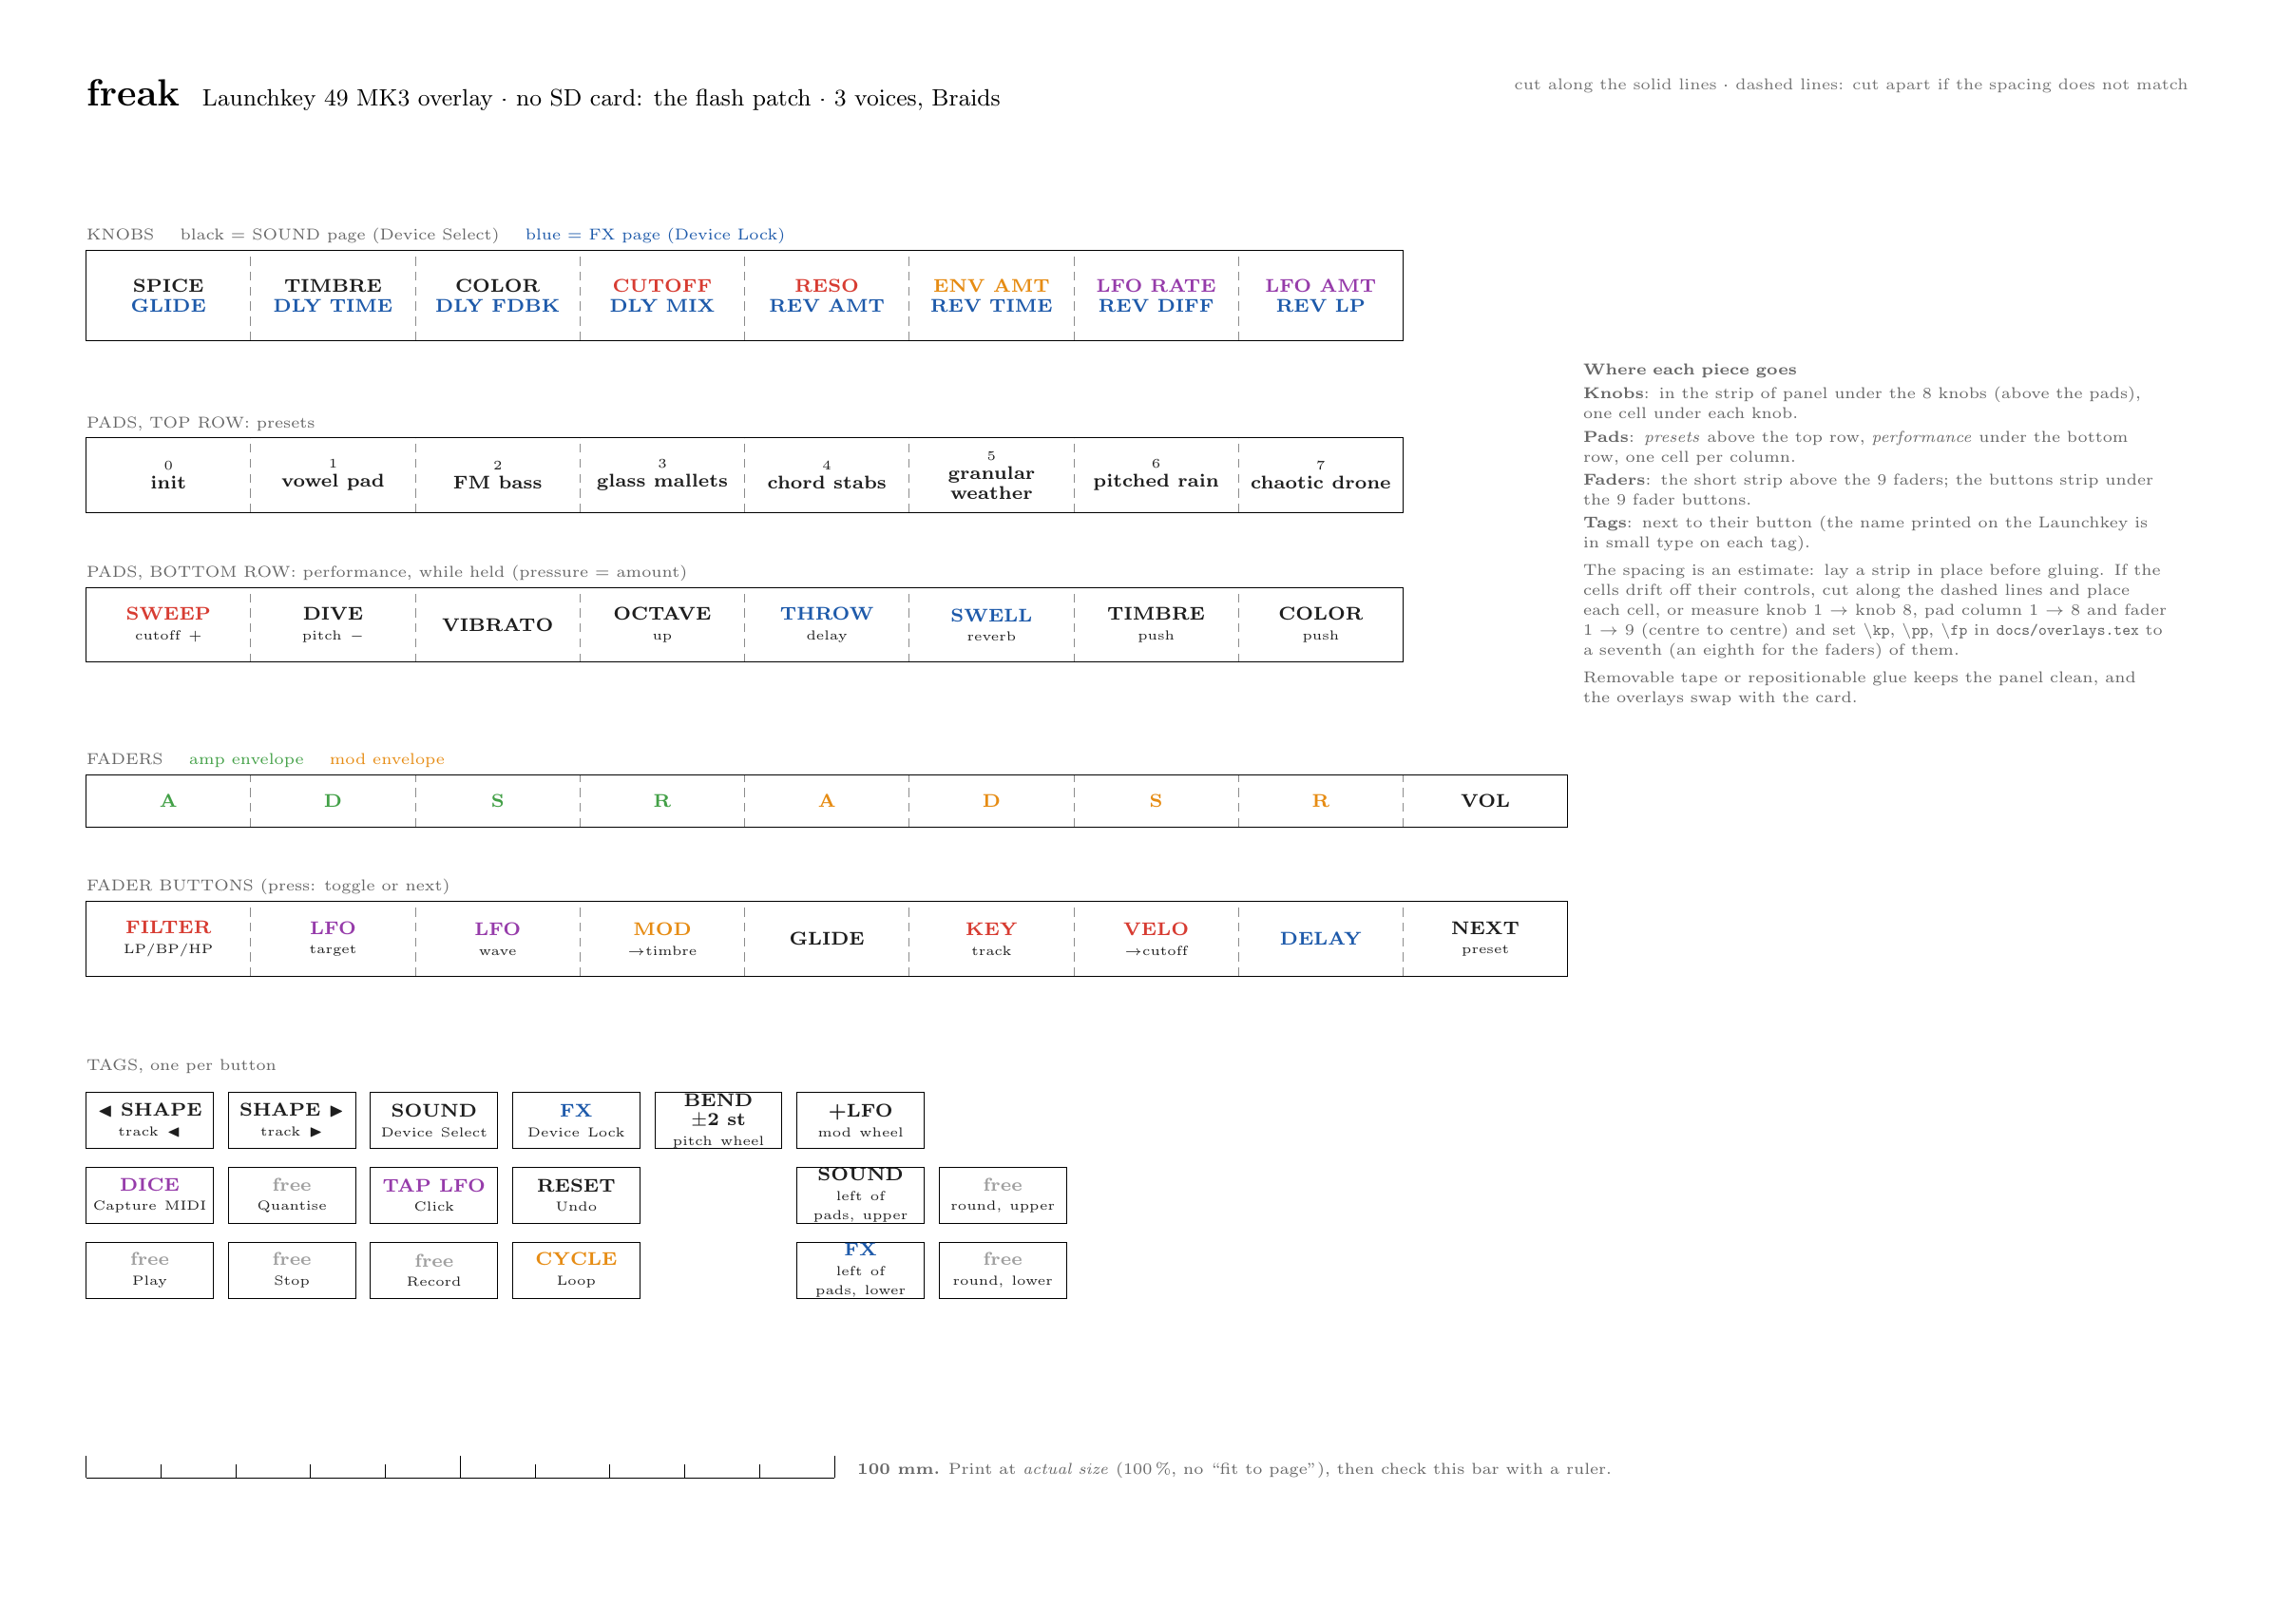
\begin{tikzpicture}[x=1mm, y=1mm]
  \useasboundingbox (0,0) rectangle (297,210);
  \header{freak}{no SD card: the flash patch \textperiodcentered{} 3 voices, Braids}

  \strip{8}{168}{8}{\kp}{12}{%
    {SPICE\\\FX{GLIDE}}, {TIMBRE\\\FX{DLY TIME}}, {COLOR\\\FX{DLY FDBK}}, {\textcolor{fltc}{CUTOFF}\\\FX{DLY MIX}},
    {\textcolor{fltc}{RESO}\\\FX{REV AMT}}, {\textcolor{modc}{ENV AMT}\\\FX{REV TIME}},
    {\textcolor{lfoc}{LFO RATE}\\\FX{REV DIFF}}, {\textcolor{lfoc}{LFO AMT}\\\FX{REV LP}}}%
    {KNOBS \quad black = SOUND page (Device Select) \quad \FX{blue = FX page (Device Lock)}}

  \strip{8}{145}{8}{\pp}{10}{%
    {\sm{0}\\init}, {\sm{1}\\vowel pad}, {\sm{2}\\FM bass}, {\sm{3}\\glass mallets}, {\sm{4}\\chord stabs}, {\sm{5}\\granular weather}, {\sm{6}\\pitched rain}, {\sm{7}\\chaotic drone}}%
    {PADS, TOP ROW: presets}
  \strip{8}{125}{8}{\pp}{10}{%
    {\textcolor{fltc}{SWEEP}\\\sm{cutoff +}}, {DIVE\\\sm{pitch \(-\)}}, {VIBRATO}, {OCTAVE\\\sm{up}},
    {\FX{THROW}\\\sm{delay}}, {\FX{SWELL}\\\sm{reverb}}, {TIMBRE\\\sm{push}}, {COLOR\\\sm{push}}}%
    {PADS, BOTTOM ROW: performance, while held (pressure = amount)}

  \strip{8}{103}{9}{\fp}{7}{%
    \textcolor{ampc}{A}, \textcolor{ampc}{D}, \textcolor{ampc}{S}, \textcolor{ampc}{R},
    \textcolor{modc}{A}, \textcolor{modc}{D}, \textcolor{modc}{S}, \textcolor{modc}{R}, VOL}%
    {FADERS \quad \textcolor{ampc}{amp envelope} \quad \textcolor{modc}{mod envelope}}
  \strip{8}{83}{9}{\fp}{10}{%
    {\textcolor{fltc}{FILTER}\\\sm{LP/BP/HP}}, {\textcolor{lfoc}{LFO}\\\sm{target}}, {\textcolor{lfoc}{LFO}\\\sm{wave}},
    {\textcolor{modc}{MOD}\\\sm{\(\to\)timbre}}, {GLIDE}, {\textcolor{fltc}{KEY}\\\sm{track}}, {\textcolor{fltc}{VELO}\\\sm{\(\to\)cutoff}},
    {\FX{DELAY}}, {NEXT\\\sm{preset}}}%
    {FADER BUTTONS (press: toggle or next)}

  \node[note, anchor=south west] at (8, 70) {TAGS, one per button};
  \tag{8}{60}{\(\blacktriangleleft\) SHAPE\\\sm{track \(\blacktriangleleft\)}}
  \tag{27}{60}{SHAPE \(\blacktriangleright\)\\\sm{track \(\blacktriangleright\)}}
  \tag{46}{60}{SOUND\\\sm{Device Select}}
  \tag{65}{60}{\FX{FX}\\\sm{Device Lock}}
  \tag{84}{60}{BEND \(\pm\)2 st\\\sm{pitch wheel}}
  \tag{103}{60}{+LFO\\\sm{mod wheel}}
  \tag{8}{50}{\textcolor{lfoc}{DICE}\\\sm{Capture MIDI}}
  \tag{27}{50}{\textcolor{freec}{free}\\\sm{Quantise}}
  \tag{46}{50}{\textcolor{lfoc}{TAP LFO}\\\sm{Click}}
  \tag{65}{50}{RESET\\\sm{Undo}}
  \tag{8}{40}{\textcolor{freec}{free}\\\sm{Play}}
  \tag{27}{40}{\textcolor{freec}{free}\\\sm{Stop}}
  \tag{46}{40}{\textcolor{freec}{free}\\\sm{Record}}
  \tag{65}{40}{\textcolor{modc}{CYCLE}\\\sm{Loop}}
  \tag{103}{50}{SOUND\\\sm{left of pads, upper}}
  \tag{103}{40}{\FX{FX}\\\sm{left of pads, lower}}
  \tag{122}{50}{\textcolor{freec}{free}\\\sm{round, upper}}
  \tag{122}{40}{\textcolor{freec}{free}\\\sm{round, lower}}

  \placement{208}{165}
  \ruler{8}{16}
\end{tikzpicture}

%======================================================================== grains
\newpage
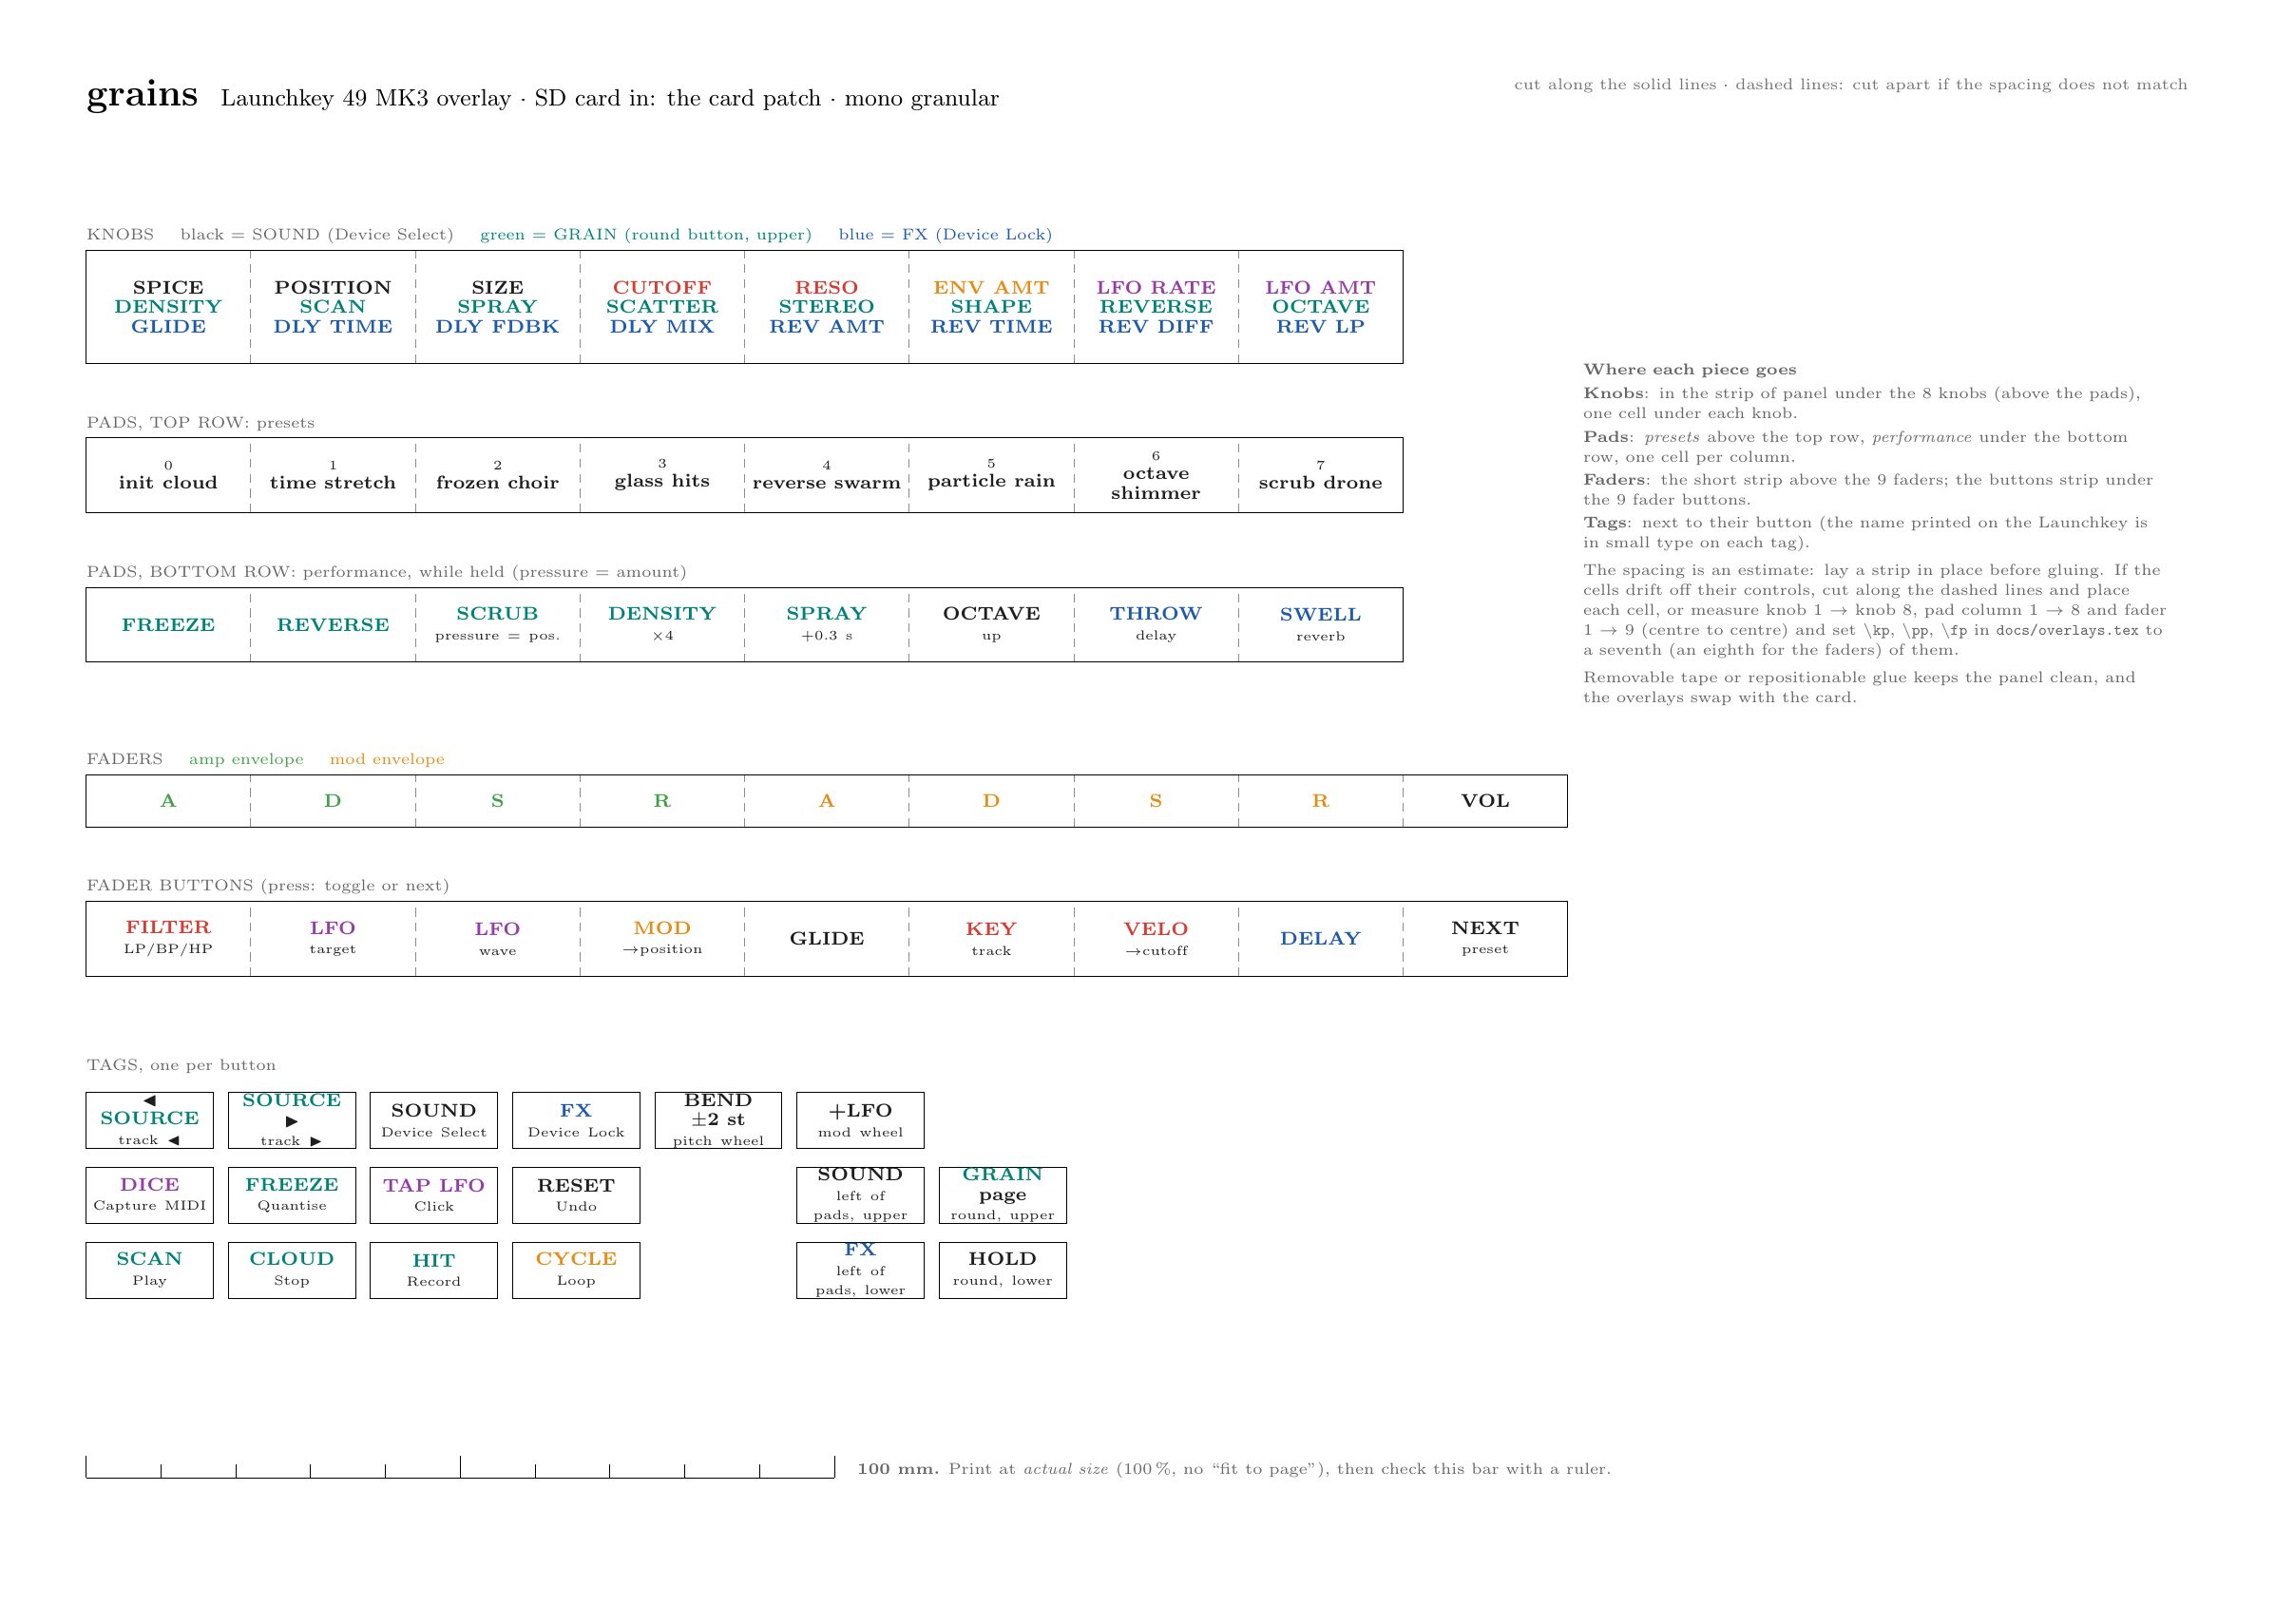
\begin{tikzpicture}[x=1mm, y=1mm]
  \useasboundingbox (0,0) rectangle (297,210);
  \header{grains}{SD card in: the card patch \textperiodcentered{} mono granular}

  \strip{8}{165}{8}{\kp}{15}{%
    {SPICE\\\GR{DENSITY}\\\FX{GLIDE}}, {POSITION\\\GR{SCAN}\\\FX{DLY TIME}}, {SIZE\\\GR{SPRAY}\\\FX{DLY FDBK}},
    {\textcolor{fltc}{CUTOFF}\\\GR{SCATTER}\\\FX{DLY MIX}}, {\textcolor{fltc}{RESO}\\\GR{STEREO}\\\FX{REV AMT}},
    {\textcolor{modc}{ENV AMT}\\\GR{SHAPE}\\\FX{REV TIME}}, {\textcolor{lfoc}{LFO RATE}\\\GR{REVERSE}\\\FX{REV DIFF}},
    {\textcolor{lfoc}{LFO AMT}\\\GR{OCTAVE}\\\FX{REV LP}}}%
    {KNOBS \quad black = SOUND (Device Select) \quad \GR{green = GRAIN (round button, upper)} \quad \FX{blue = FX (Device Lock)}}

  \strip{8}{145}{8}{\pp}{10}{%
    {\sm{0}\\init cloud}, {\sm{1}\\time stretch}, {\sm{2}\\frozen choir}, {\sm{3}\\glass hits}, {\sm{4}\\reverse swarm}, {\sm{5}\\particle rain},
    {\sm{6}\\octave shimmer}, {\sm{7}\\scrub drone}}%
    {PADS, TOP ROW: presets}
  \strip{8}{125}{8}{\pp}{10}{%
    {\GR{FREEZE}}, {\GR{REVERSE}}, {\GR{SCRUB}\\\sm{pressure = pos.}}, {\GR{DENSITY}\\\sm{\(\times\)4}},
    {\GR{SPRAY}\\\sm{+0.3 s}}, {OCTAVE\\\sm{up}}, {\FX{THROW}\\\sm{delay}}, {\FX{SWELL}\\\sm{reverb}}}%
    {PADS, BOTTOM ROW: performance, while held (pressure = amount)}

  \strip{8}{103}{9}{\fp}{7}{%
    \textcolor{ampc}{A}, \textcolor{ampc}{D}, \textcolor{ampc}{S}, \textcolor{ampc}{R},
    \textcolor{modc}{A}, \textcolor{modc}{D}, \textcolor{modc}{S}, \textcolor{modc}{R}, VOL}%
    {FADERS \quad \textcolor{ampc}{amp envelope} \quad \textcolor{modc}{mod envelope}}
  \strip{8}{83}{9}{\fp}{10}{%
    {\textcolor{fltc}{FILTER}\\\sm{LP/BP/HP}}, {\textcolor{lfoc}{LFO}\\\sm{target}}, {\textcolor{lfoc}{LFO}\\\sm{wave}},
    {\textcolor{modc}{MOD}\\\sm{\(\to\)position}}, {GLIDE}, {\textcolor{fltc}{KEY}\\\sm{track}}, {\textcolor{fltc}{VELO}\\\sm{\(\to\)cutoff}},
    {\FX{DELAY}}, {NEXT\\\sm{preset}}}%
    {FADER BUTTONS (press: toggle or next)}

  \node[note, anchor=south west] at (8, 70) {TAGS, one per button};
  \tag{8}{60}{\(\blacktriangleleft\) \GR{SOURCE}\\\sm{track \(\blacktriangleleft\)}}
  \tag{27}{60}{\GR{SOURCE} \(\blacktriangleright\)\\\sm{track \(\blacktriangleright\)}}
  \tag{46}{60}{SOUND\\\sm{Device Select}}
  \tag{65}{60}{\FX{FX}\\\sm{Device Lock}}
  \tag{84}{60}{BEND \(\pm\)2 st\\\sm{pitch wheel}}
  \tag{103}{60}{+LFO\\\sm{mod wheel}}
  \tag{8}{50}{\textcolor{lfoc}{DICE}\\\sm{Capture MIDI}}
  \tag{27}{50}{\GR{FREEZE}\\\sm{Quantise}}
  \tag{46}{50}{\textcolor{lfoc}{TAP LFO}\\\sm{Click}}
  \tag{65}{50}{RESET\\\sm{Undo}}
  \tag{8}{40}{\GR{SCAN}\\\sm{Play}}
  \tag{27}{40}{\GR{CLOUD}\\\sm{Stop}}
  \tag{46}{40}{\GR{HIT}\\\sm{Record}}
  \tag{65}{40}{\textcolor{modc}{CYCLE}\\\sm{Loop}}
  \tag{103}{50}{SOUND\\\sm{left of pads, upper}}
  \tag{103}{40}{\FX{FX}\\\sm{left of pads, lower}}
  \tag{122}{50}{\GR{GRAIN} page\\\sm{round, upper}}
  \tag{122}{40}{HOLD\\\sm{round, lower}}

  \placement{208}{165}
  \ruler{8}{16}
\end{tikzpicture}

%======================================================================== groove
\newpage
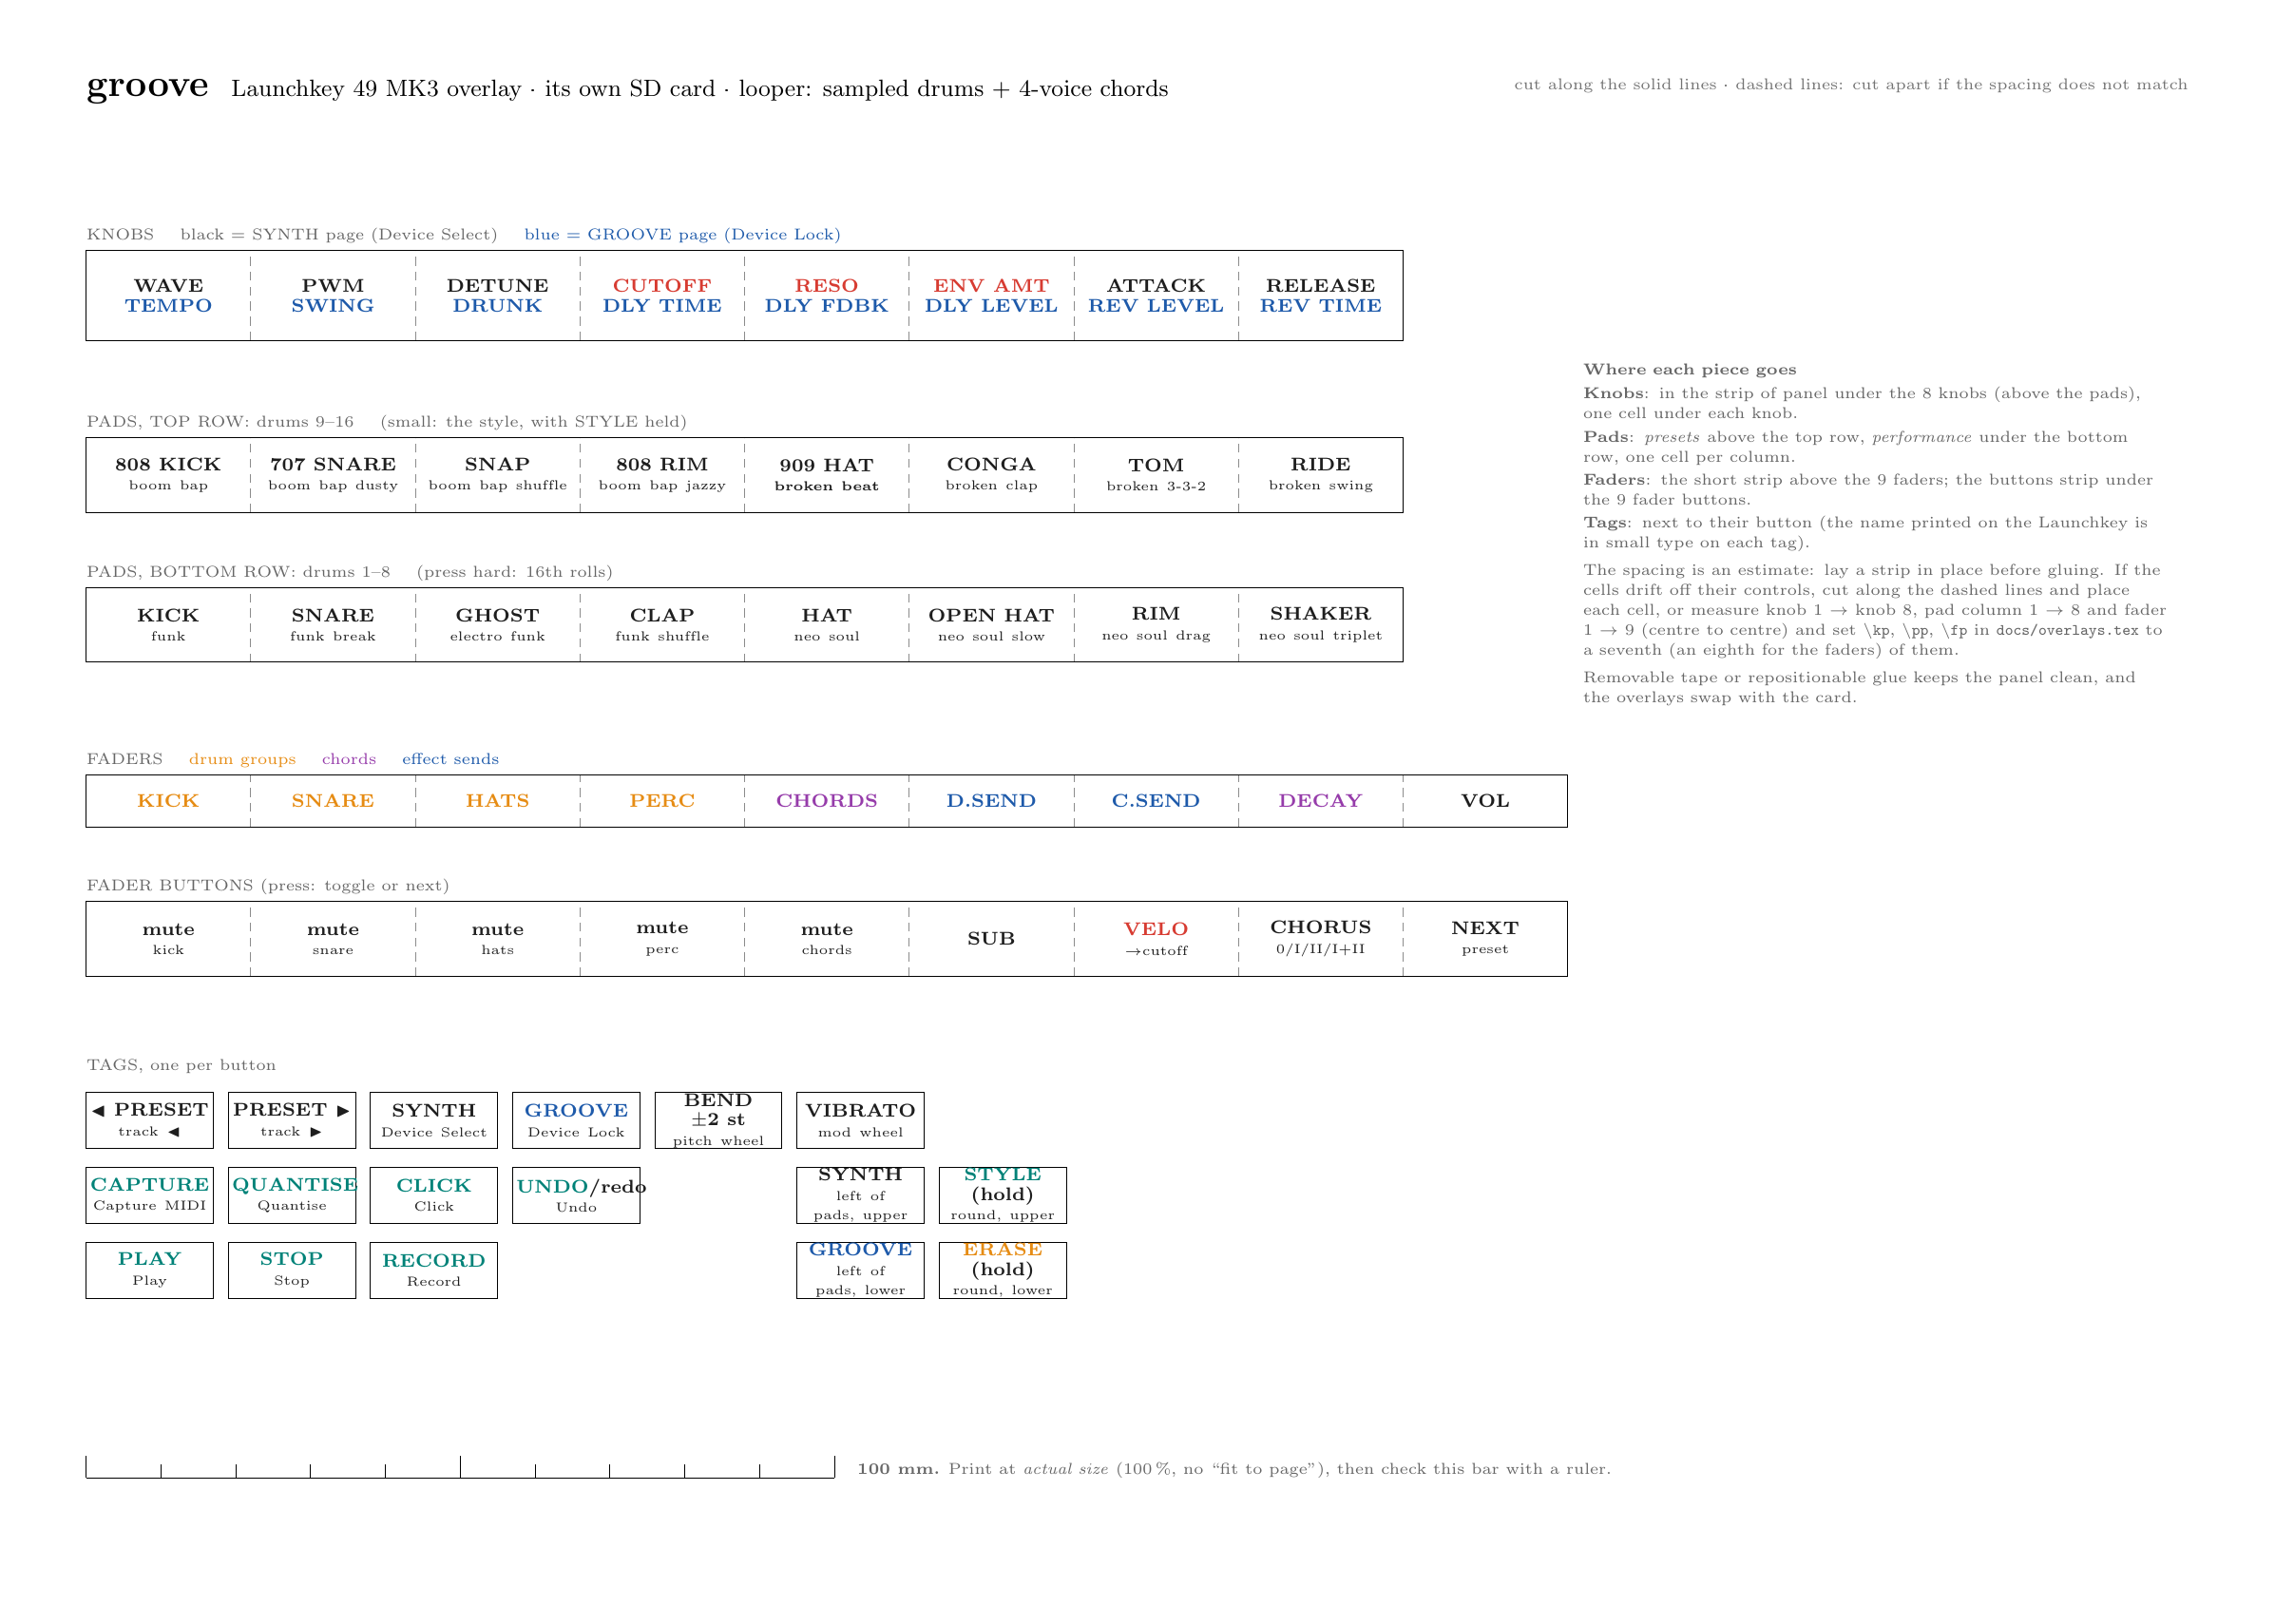
\begin{tikzpicture}[x=1mm, y=1mm]
  \useasboundingbox (0,0) rectangle (297,210);
  \header{groove}{its own SD card \textperiodcentered{} looper: sampled drums + 4-voice chords}

  \strip{8}{168}{8}{\kp}{12}{%
    {WAVE\\\FX{TEMPO}}, {PWM\\\FX{SWING}}, {DETUNE\\\FX{DRUNK}}, {\textcolor{fltc}{CUTOFF}\\\FX{DLY TIME}},
    {\textcolor{fltc}{RESO}\\\FX{DLY FDBK}}, {\textcolor{fltc}{ENV AMT}\\\FX{DLY LEVEL}},
    {ATTACK\\\FX{REV LEVEL}}, {RELEASE\\\FX{REV TIME}}}%
    {KNOBS \quad black = SYNTH page (Device Select) \quad \FX{blue = GROOVE page (Device Lock)}}

  \strip{8}{145}{8}{\pp}{10}{%
    {808 KICK\\\sm{boom bap}}, {707 SNARE\\\sm{boom bap dusty}}, {SNAP\\\sm{boom bap shuffle}}, {808 RIM\\\sm{boom bap jazzy}},
    {909 HAT\\\sm{\textbf{broken beat}}}, {CONGA\\\sm{broken clap}}, {TOM\\\sm{broken 3-3-2}}, {RIDE\\\sm{broken swing}}}%
    {PADS, TOP ROW: drums 9--16 \quad (small: the style, with STYLE held)}
  \strip{8}{125}{8}{\pp}{10}{%
    {KICK\\\sm{funk}}, {SNARE\\\sm{funk break}}, {GHOST\\\sm{electro funk}}, {CLAP\\\sm{funk shuffle}},
    {HAT\\\sm{neo soul}}, {OPEN HAT\\\sm{neo soul slow}}, {RIM\\\sm{neo soul drag}}, {SHAKER\\\sm{neo soul triplet}}}%
    {PADS, BOTTOM ROW: drums 1--8 \quad (press hard: 16th rolls)}

  \strip{8}{103}{9}{\fp}{7}{%
    \textcolor{modc}{KICK}, \textcolor{modc}{SNARE}, \textcolor{modc}{HATS}, \textcolor{modc}{PERC},
    \textcolor{lfoc}{CHORDS}, \FX{D.SEND}, \FX{C.SEND}, \textcolor{lfoc}{DECAY}, VOL}%
    {FADERS \quad \textcolor{modc}{drum groups} \quad \textcolor{lfoc}{chords} \quad \FX{effect sends}}
  \strip{8}{83}{9}{\fp}{10}{%
    {mute\\\sm{kick}}, {mute\\\sm{snare}}, {mute\\\sm{hats}}, {mute\\\sm{perc}}, {mute\\\sm{chords}},
    {SUB}, {\textcolor{fltc}{VELO}\\\sm{\(\to\)cutoff}}, {CHORUS\\\sm{0/I/II/I+II}}, {NEXT\\\sm{preset}}}%
    {FADER BUTTONS (press: toggle or next)}

  \node[note, anchor=south west] at (8, 70) {TAGS, one per button};
  \tag{8}{60}{\(\blacktriangleleft\) PRESET\\\sm{track \(\blacktriangleleft\)}}
  \tag{27}{60}{PRESET \(\blacktriangleright\)\\\sm{track \(\blacktriangleright\)}}
  \tag{46}{60}{SYNTH\\\sm{Device Select}}
  \tag{65}{60}{\FX{GROOVE}\\\sm{Device Lock}}
  \tag{84}{60}{BEND \(\pm\)2 st\\\sm{pitch wheel}}
  \tag{103}{60}{VIBRATO\\\sm{mod wheel}}
  \tag{8}{50}{\GR{CAPTURE}\\\sm{Capture MIDI}}
  \tag{27}{50}{\GR{QUANTISE}\\\sm{Quantise}}
  \tag{46}{50}{\GR{CLICK}\\\sm{Click}}
  \tag{65}{50}{\GR{UNDO}/redo\\\sm{Undo}}
  \tag{8}{40}{\GR{PLAY}\\\sm{Play}}
  \tag{27}{40}{\GR{STOP}\\\sm{Stop}}
  \tag{46}{40}{\GR{RECORD}\\\sm{Record}}
  \tag{103}{50}{SYNTH\\\sm{left of pads, upper}}
  \tag{103}{40}{\FX{GROOVE}\\\sm{left of pads, lower}}
  \tag{122}{50}{\GR{STYLE} (hold)\\\sm{round, upper}}
  \tag{122}{40}{\textcolor{modc}{ERASE} (hold)\\\sm{round, lower}}

  \placement{208}{165}
  \ruler{8}{16}
\end{tikzpicture}

%======================================================================== soliton
\newpage
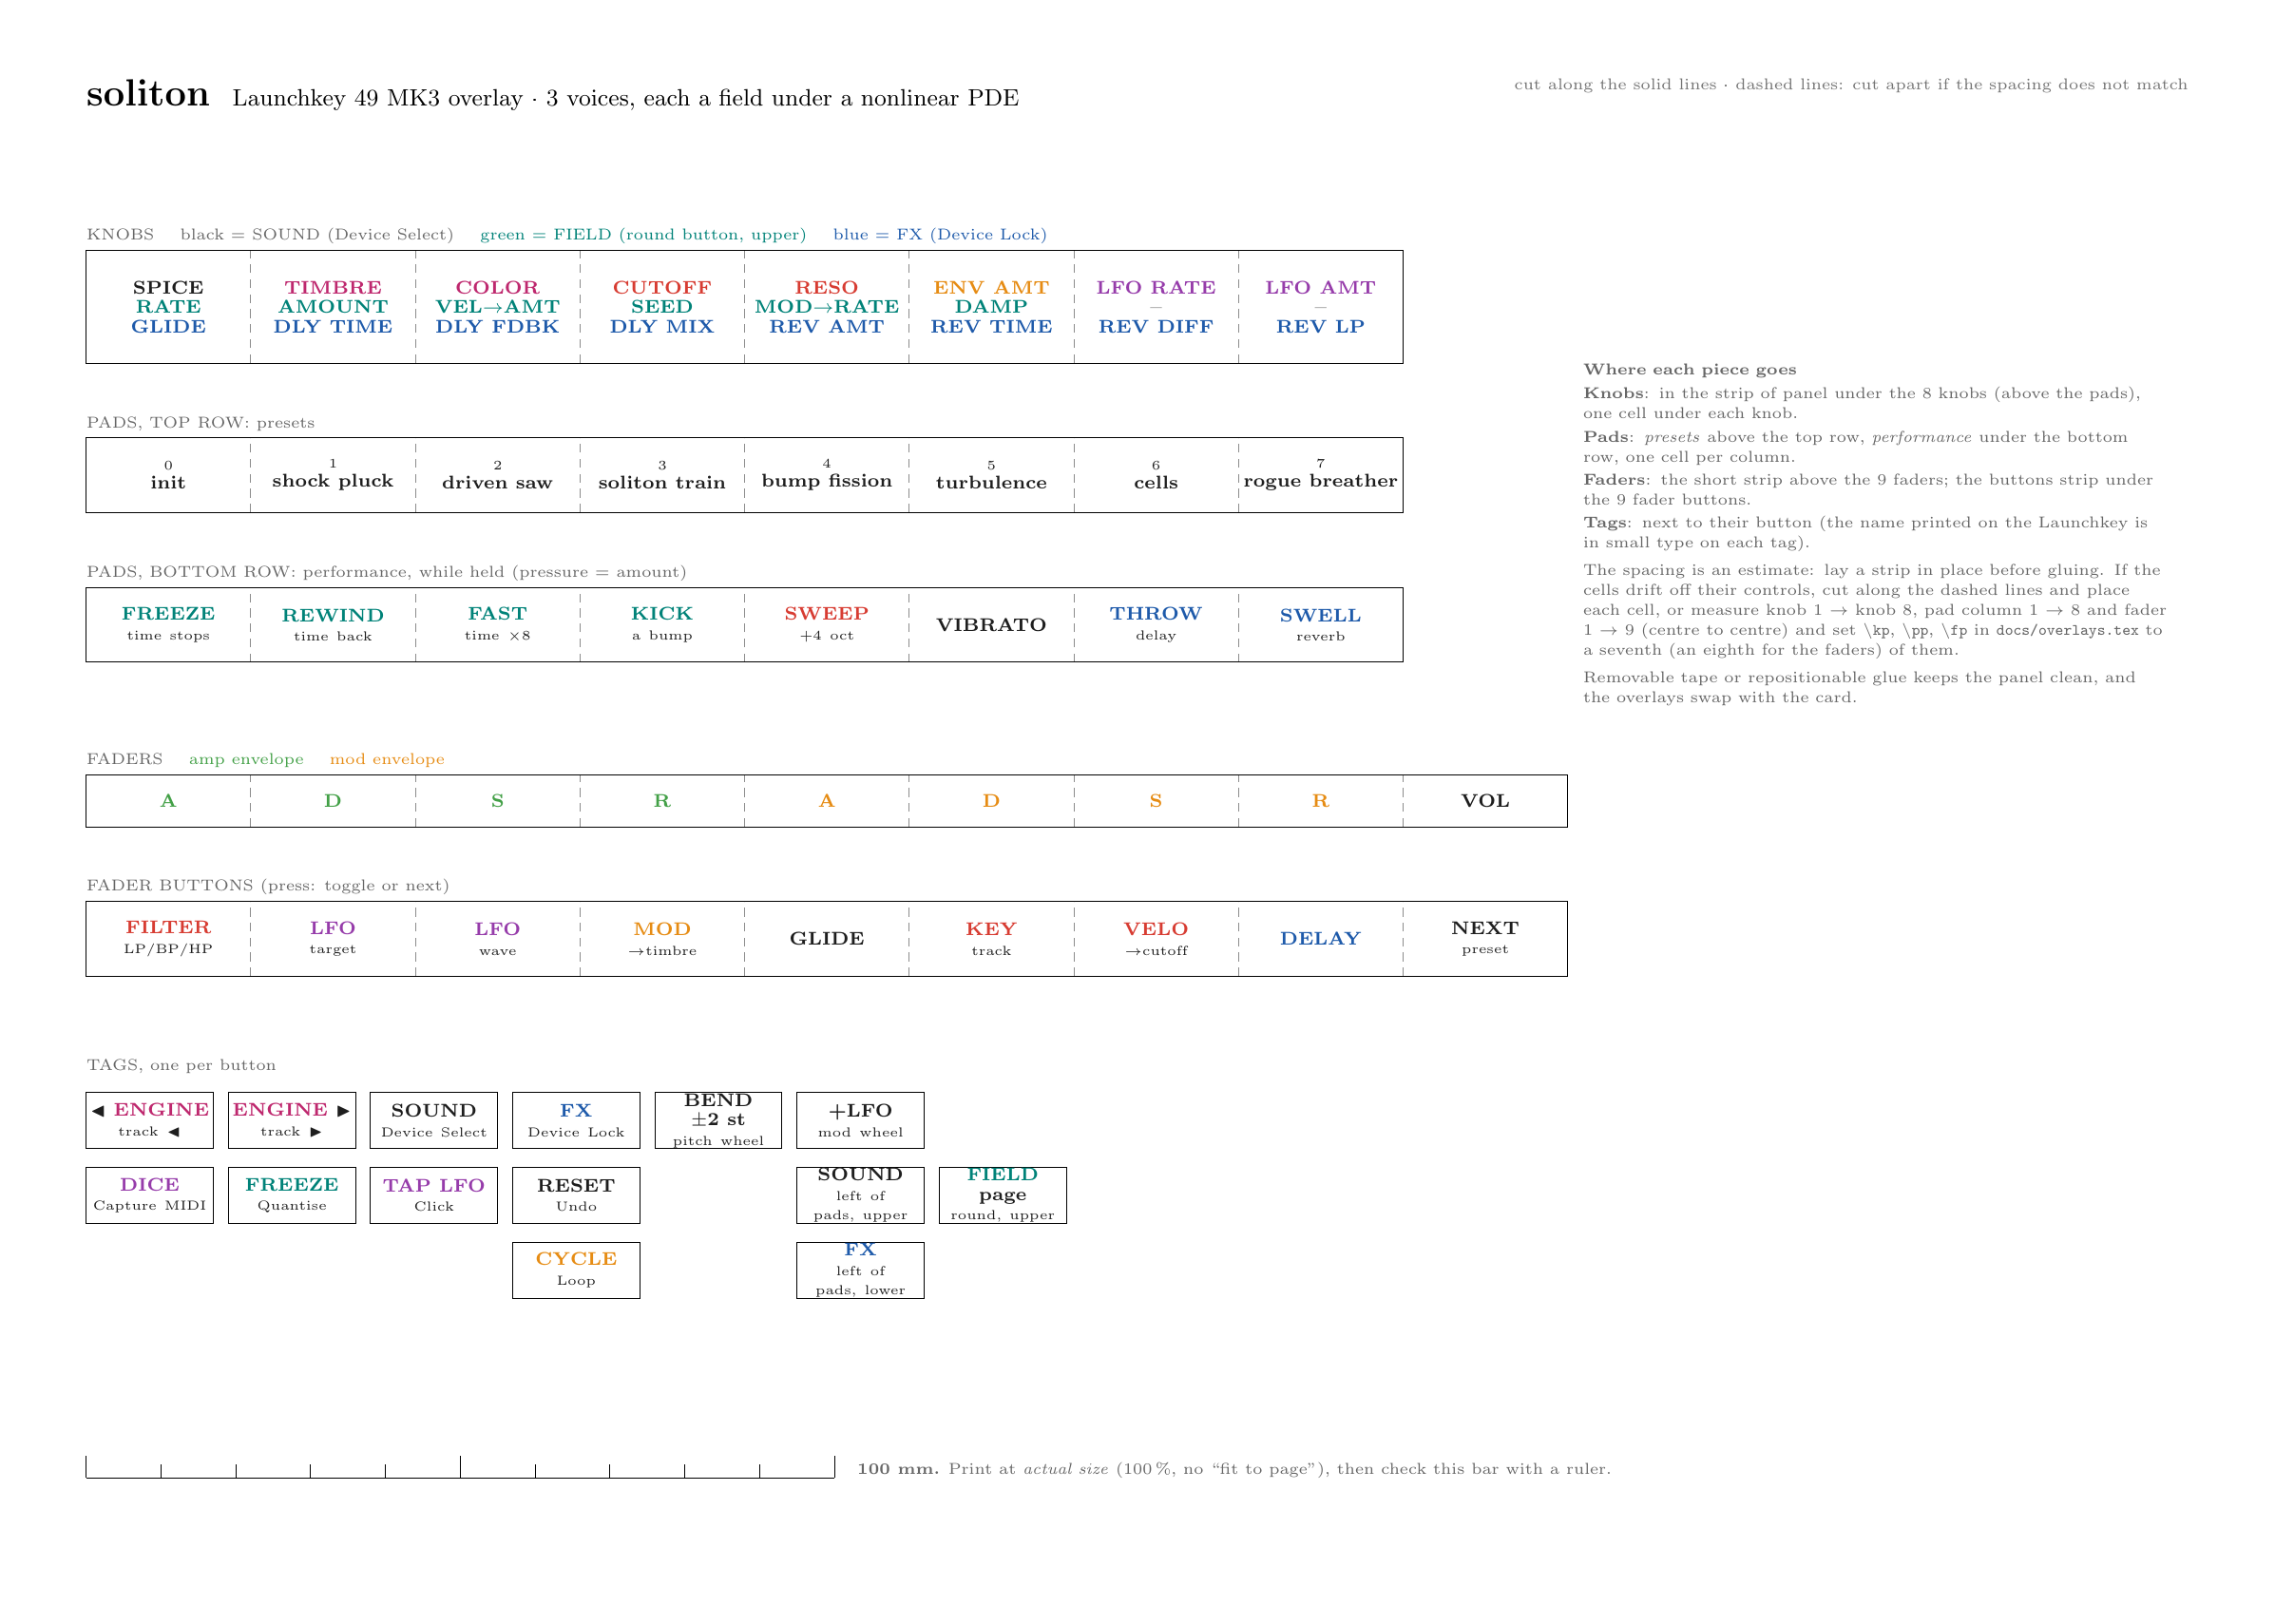
\begin{tikzpicture}[x=1mm, y=1mm]
  \useasboundingbox (0,0) rectangle (297,210);
  \header{soliton}{3 voices, each a field under a nonlinear PDE}

  \strip{8}{165}{8}{\kp}{15}{%
    {SPICE\\\GR{RATE}\\\FX{GLIDE}}, {\textcolor{engc}{TIMBRE}\\\GR{AMOUNT}\\\FX{DLY TIME}}, {\textcolor{engc}{COLOR}\\\GR{VEL\(\to\)AMT}\\\FX{DLY FDBK}},
    {\textcolor{fltc}{CUTOFF}\\\GR{SEED}\\\FX{DLY MIX}}, {\textcolor{fltc}{RESO}\\\GR{MOD\(\to\)RATE}\\\FX{REV AMT}},
    {\textcolor{modc}{ENV AMT}\\\GR{DAMP}\\\FX{REV TIME}}, {\textcolor{lfoc}{LFO RATE}\\\textcolor{freec}{--}\\\FX{REV DIFF}},
    {\textcolor{lfoc}{LFO AMT}\\\textcolor{freec}{--}\\\FX{REV LP}}}%
    {KNOBS \quad black = SOUND (Device Select) \quad \GR{green = FIELD (round button, upper)} \quad \FX{blue = FX (Device Lock)}}

  \strip{8}{145}{8}{\pp}{10}{%
    {\sm{0}\\init}, {\sm{1}\\shock pluck}, {\sm{2}\\driven saw}, {\sm{3}\\soliton train}, {\sm{4}\\bump fission}, {\sm{5}\\turbulence},
    {\sm{6}\\cells}, {\sm{7}\\rogue breather}}%
    {PADS, TOP ROW: presets}
  \strip{8}{125}{8}{\pp}{10}{%
    {\GR{FREEZE}\\\sm{time stops}}, {\GR{REWIND}\\\sm{time back}}, {\GR{FAST}\\\sm{time \(\times\)8}}, {\GR{KICK}\\\sm{a bump}},
    {\textcolor{fltc}{SWEEP}\\\sm{+4 oct}}, {VIBRATO}, {\FX{THROW}\\\sm{delay}}, {\FX{SWELL}\\\sm{reverb}}}%
    {PADS, BOTTOM ROW: performance, while held (pressure = amount)}

  \strip{8}{103}{9}{\fp}{7}{%
    \textcolor{ampc}{A}, \textcolor{ampc}{D}, \textcolor{ampc}{S}, \textcolor{ampc}{R},
    \textcolor{modc}{A}, \textcolor{modc}{D}, \textcolor{modc}{S}, \textcolor{modc}{R}, VOL}%
    {FADERS \quad \textcolor{ampc}{amp envelope} \quad \textcolor{modc}{mod envelope}}
  \strip{8}{83}{9}{\fp}{10}{%
    {\textcolor{fltc}{FILTER}\\\sm{LP/BP/HP}}, {\textcolor{lfoc}{LFO}\\\sm{target}}, {\textcolor{lfoc}{LFO}\\\sm{wave}},
    {\textcolor{modc}{MOD}\\\sm{\(\to\)timbre}}, {GLIDE}, {\textcolor{fltc}{KEY}\\\sm{track}}, {\textcolor{fltc}{VELO}\\\sm{\(\to\)cutoff}},
    {\FX{DELAY}}, {NEXT\\\sm{preset}}}%
    {FADER BUTTONS (press: toggle or next)}

  \node[note, anchor=south west] at (8, 70) {TAGS, one per button};
  \tag{8}{60}{\(\blacktriangleleft\) \textcolor{engc}{ENGINE}\\\sm{track \(\blacktriangleleft\)}}
  \tag{27}{60}{\textcolor{engc}{ENGINE} \(\blacktriangleright\)\\\sm{track \(\blacktriangleright\)}}
  \tag{46}{60}{SOUND\\\sm{Device Select}}
  \tag{65}{60}{\FX{FX}\\\sm{Device Lock}}
  \tag{84}{60}{BEND \(\pm\)2 st\\\sm{pitch wheel}}
  \tag{103}{60}{+LFO\\\sm{mod wheel}}
  \tag{8}{50}{\textcolor{lfoc}{DICE}\\\sm{Capture MIDI}}
  \tag{27}{50}{\GR{FREEZE}\\\sm{Quantise}}
  \tag{46}{50}{\textcolor{lfoc}{TAP LFO}\\\sm{Click}}
  \tag{65}{50}{RESET\\\sm{Undo}}
  \tag{65}{40}{\textcolor{modc}{CYCLE}\\\sm{Loop}}
  \tag{103}{50}{SOUND\\\sm{left of pads, upper}}
  \tag{103}{40}{\FX{FX}\\\sm{left of pads, lower}}
  \tag{122}{50}{\GR{FIELD} page\\\sm{round, upper}}

  \placement{208}{165}
  \ruler{8}{16}
\end{tikzpicture}

%======================================================================== aeolian
\newpage
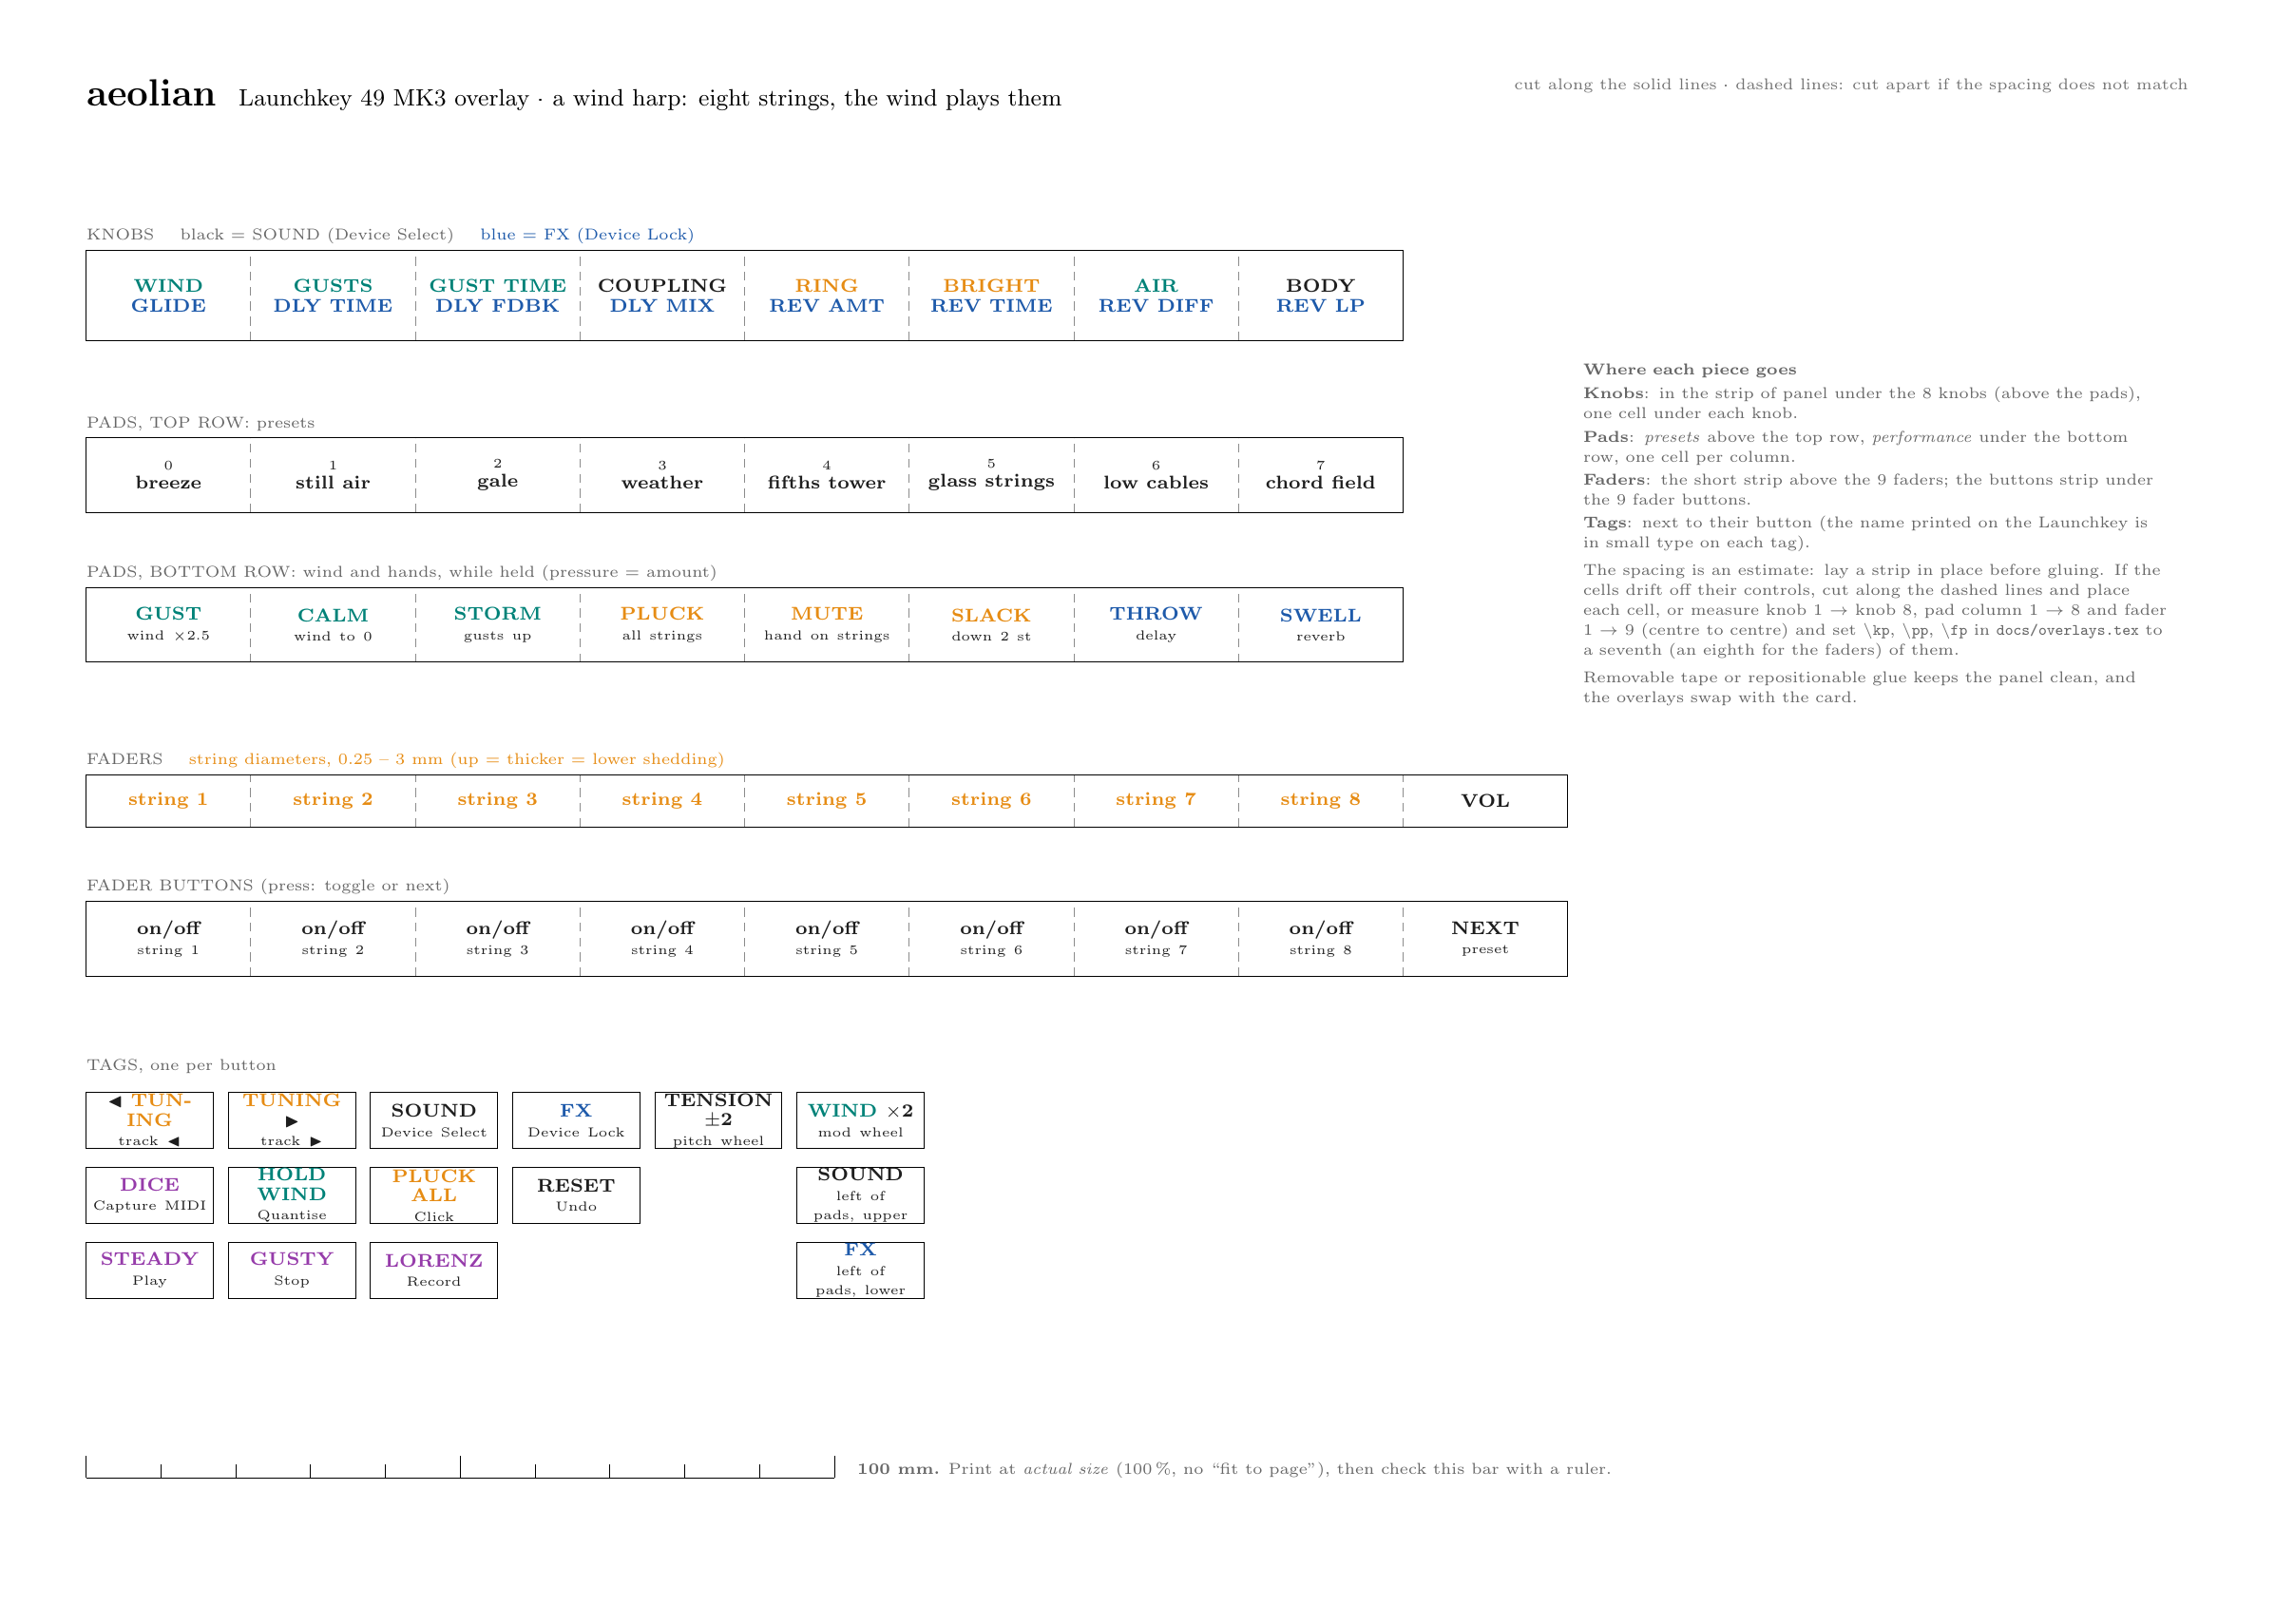
\begin{tikzpicture}[x=1mm, y=1mm]
  \useasboundingbox (0,0) rectangle (297,210);
  \header{aeolian}{a wind harp: eight strings, the wind plays them}

  \strip{8}{168}{8}{\kp}{12}{%
    {\GR{WIND}\\\FX{GLIDE}}, {\GR{GUSTS}\\\FX{DLY TIME}}, {\GR{GUST TIME}\\\FX{DLY FDBK}}, {COUPLING\\\FX{DLY MIX}},
    {\textcolor{modc}{RING}\\\FX{REV AMT}}, {\textcolor{modc}{BRIGHT}\\\FX{REV TIME}}, {\GR{AIR}\\\FX{REV DIFF}}, {BODY\\\FX{REV LP}}}%
    {KNOBS \quad black = SOUND (Device Select) \quad \FX{blue = FX (Device Lock)}}

  \strip{8}{145}{8}{\pp}{10}{%
    {\sm{0}\\breeze}, {\sm{1}\\still air}, {\sm{2}\\gale}, {\sm{3}\\weather}, {\sm{4}\\fifths tower}, {\sm{5}\\glass strings},
    {\sm{6}\\low cables}, {\sm{7}\\chord field}}%
    {PADS, TOP ROW: presets}
  \strip{8}{125}{8}{\pp}{10}{%
    {\GR{GUST}\\\sm{wind \(\times\)2.5}}, {\GR{CALM}\\\sm{wind to 0}}, {\GR{STORM}\\\sm{gusts up}}, {\textcolor{modc}{PLUCK}\\\sm{all strings}},
    {\textcolor{modc}{MUTE}\\\sm{hand on strings}}, {\textcolor{modc}{SLACK}\\\sm{down 2 st}}, {\FX{THROW}\\\sm{delay}}, {\FX{SWELL}\\\sm{reverb}}}%
    {PADS, BOTTOM ROW: wind and hands, while held (pressure = amount)}

  \strip{8}{103}{9}{\fp}{7}{%
    \textcolor{modc}{string 1}, \textcolor{modc}{string 2}, \textcolor{modc}{string 3}, \textcolor{modc}{string 4},
    \textcolor{modc}{string 5}, \textcolor{modc}{string 6}, \textcolor{modc}{string 7}, \textcolor{modc}{string 8}, VOL}%
    {FADERS \quad \textcolor{modc}{string diameters, 0.25 -- 3 mm (up = thicker = lower shedding)}}
  \strip{8}{83}{9}{\fp}{10}{%
    {on/off\\\sm{string 1}}, {on/off\\\sm{string 2}}, {on/off\\\sm{string 3}}, {on/off\\\sm{string 4}}, {on/off\\\sm{string 5}},
    {on/off\\\sm{string 6}}, {on/off\\\sm{string 7}}, {on/off\\\sm{string 8}}, {NEXT\\\sm{preset}}}%
    {FADER BUTTONS (press: toggle or next)}

  \node[note, anchor=south west] at (8, 70) {TAGS, one per button};
  \tag{8}{60}{\(\blacktriangleleft\) \textcolor{modc}{TUNING}\\\sm{track \(\blacktriangleleft\)}}
  \tag{27}{60}{\textcolor{modc}{TUNING} \(\blacktriangleright\)\\\sm{track \(\blacktriangleright\)}}
  \tag{46}{60}{SOUND\\\sm{Device Select}}
  \tag{65}{60}{\FX{FX}\\\sm{Device Lock}}
  \tag{84}{60}{TENSION \(\pm\)2\\\sm{pitch wheel}}
  \tag{103}{60}{\GR{WIND} \(\times\)2\\\sm{mod wheel}}
  \tag{8}{50}{\textcolor{lfoc}{DICE}\\\sm{Capture MIDI}}
  \tag{27}{50}{\GR{HOLD WIND}\\\sm{Quantise}}
  \tag{46}{50}{\textcolor{modc}{PLUCK ALL}\\\sm{Click}}
  \tag{65}{50}{RESET\\\sm{Undo}}
  \tag{8}{40}{\textcolor{lfoc}{STEADY}\\\sm{Play}}
  \tag{27}{40}{\textcolor{lfoc}{GUSTY}\\\sm{Stop}}
  \tag{46}{40}{\textcolor{lfoc}{LORENZ}\\\sm{Record}}
  \tag{103}{50}{SOUND\\\sm{left of pads, upper}}
  \tag{103}{40}{\FX{FX}\\\sm{left of pads, lower}}

  \placement{208}{165}
  \ruler{8}{16}
\end{tikzpicture}

%======================================================================== raw
\newpage
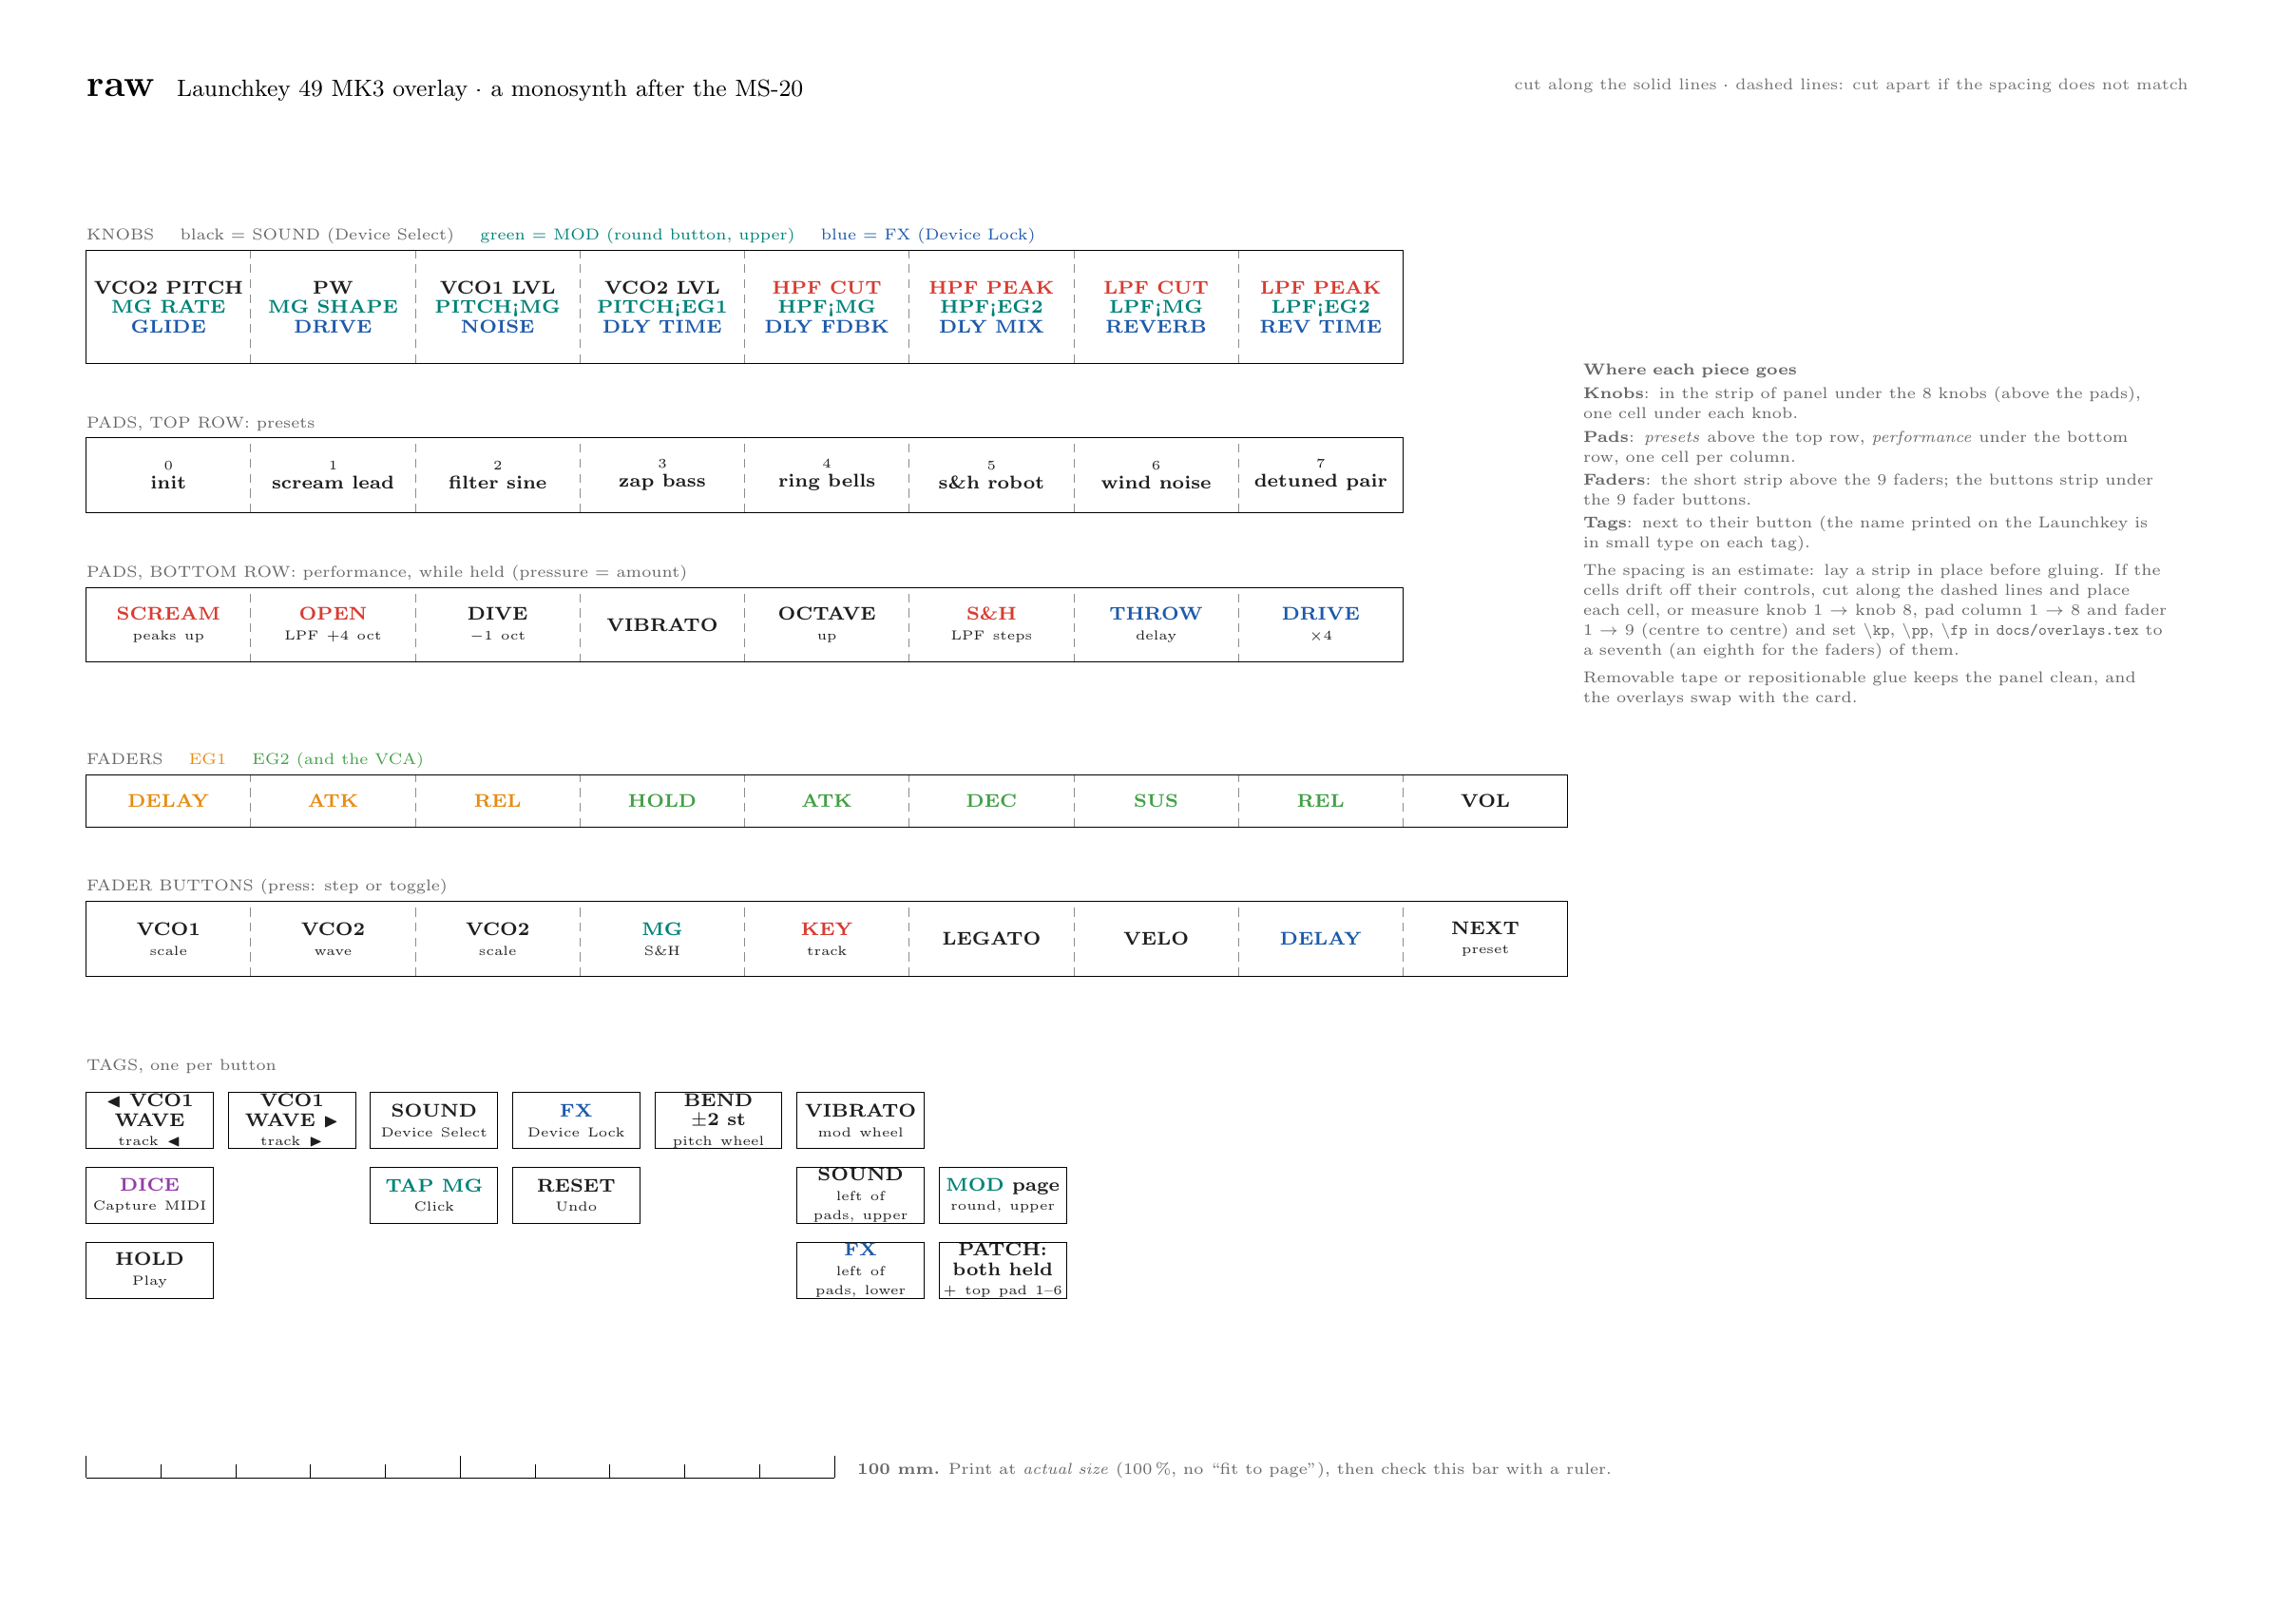
\begin{tikzpicture}[x=1mm, y=1mm]
  \useasboundingbox (0,0) rectangle (297,210);
  \header{raw}{a monosynth after the MS-20}

  \strip{8}{165}{8}{\kp}{15}{%
    {VCO2 PITCH\\\GR{MG RATE}\\\FX{GLIDE}}, {PW\\\GR{MG SHAPE}\\\FX{DRIVE}}, {VCO1 LVL\\\GR{PITCH<MG}\\\FX{NOISE}},
    {VCO2 LVL\\\GR{PITCH<EG1}\\\FX{DLY TIME}}, {\textcolor{fltc}{HPF CUT}\\\GR{HPF<MG}\\\FX{DLY FDBK}},
    {\textcolor{fltc}{HPF PEAK}\\\GR{HPF<EG2}\\\FX{DLY MIX}}, {\textcolor{fltc}{LPF CUT}\\\GR{LPF<MG}\\\FX{REVERB}},
    {\textcolor{fltc}{LPF PEAK}\\\GR{LPF<EG2}\\\FX{REV TIME}}}%
    {KNOBS \quad black = SOUND (Device Select) \quad \GR{green = MOD (round button, upper)} \quad \FX{blue = FX (Device Lock)}}

  \strip{8}{145}{8}{\pp}{10}{%
    {\sm{0}\\init}, {\sm{1}\\scream lead}, {\sm{2}\\filter sine}, {\sm{3}\\zap bass}, {\sm{4}\\ring bells}, {\sm{5}\\s\&h robot},
    {\sm{6}\\wind noise}, {\sm{7}\\detuned pair}}%
    {PADS, TOP ROW: presets}
  \strip{8}{125}{8}{\pp}{10}{%
    {\textcolor{fltc}{SCREAM}\\\sm{peaks up}}, {\textcolor{fltc}{OPEN}\\\sm{LPF +4 oct}}, {DIVE\\\sm{\(-\)1 oct}}, {VIBRATO},
    {OCTAVE\\\sm{up}}, {\textcolor{fltc}{S\&H}\\\sm{LPF steps}}, {\FX{THROW}\\\sm{delay}}, {\FX{DRIVE}\\\sm{\(\times\)4}}}%
    {PADS, BOTTOM ROW: performance, while held (pressure = amount)}

  \strip{8}{103}{9}{\fp}{7}{%
    \textcolor{modc}{DELAY}, \textcolor{modc}{ATK}, \textcolor{modc}{REL},
    \textcolor{ampc}{HOLD}, \textcolor{ampc}{ATK}, \textcolor{ampc}{DEC}, \textcolor{ampc}{SUS}, \textcolor{ampc}{REL}, VOL}%
    {FADERS \quad \textcolor{modc}{EG1} \quad \textcolor{ampc}{EG2 (and the VCA)}}
  \strip{8}{83}{9}{\fp}{10}{%
    {VCO1\\\sm{scale}}, {VCO2\\\sm{wave}}, {VCO2\\\sm{scale}}, {\GR{MG}\\\sm{S\&H}}, {\textcolor{fltc}{KEY}\\\sm{track}},
    {LEGATO}, {VELO}, {\FX{DELAY}}, {NEXT\\\sm{preset}}}%
    {FADER BUTTONS (press: step or toggle)}

  \node[note, anchor=south west] at (8, 70) {TAGS, one per button};
  \tag{8}{60}{\(\blacktriangleleft\) VCO1 WAVE\\\sm{track \(\blacktriangleleft\)}}
  \tag{27}{60}{VCO1 WAVE \(\blacktriangleright\)\\\sm{track \(\blacktriangleright\)}}
  \tag{46}{60}{SOUND\\\sm{Device Select}}
  \tag{65}{60}{\FX{FX}\\\sm{Device Lock}}
  \tag{84}{60}{BEND \(\pm\)2 st\\\sm{pitch wheel}}
  \tag{103}{60}{VIBRATO\\\sm{mod wheel}}
  \tag{8}{50}{\textcolor{lfoc}{DICE}\\\sm{Capture MIDI}}
  \tag{46}{50}{\GR{TAP MG}\\\sm{Click}}
  \tag{65}{50}{RESET\\\sm{Undo}}
  \tag{8}{40}{HOLD\\\sm{Play}}
  \tag{103}{50}{SOUND\\\sm{left of pads, upper}}
  \tag{103}{40}{\FX{FX}\\\sm{left of pads, lower}}
  \tag{122}{40}{PATCH: both held\\\sm{+ top pad 1--6}}
  \tag{122}{50}{\GR{MOD} page\\\sm{round, upper}}

  \placement{208}{165}
  \ruler{8}{16}
\end{tikzpicture}
\end{document}
